% Source: book pp. 182--196 (PDF 196--210); no solutions.
% Numbered equations (6.15, 6.18, ...): \axeqstep{ax:N.M} steps Axler's counter
% and sets the label just before the display; \axeqtag prints the number.
\providecommand\axeqstep[1]{\refstepcounter{theorem}\label{#1}}
\providecommand\axeqtag{\tag*{\thetheorem}}
\section{Inner Products and Norms}

\subsection{Inner Products}

\marginfig{\begin{tikzpicture}[scale=.6]
  \draw[axis] (-.3,0)--(4,0); \draw[axis] (0,-.3)--(0,2);
  \draw[vec] (0,0)--node[above left=-2pt,font=\scriptsize]{$v$} (3.1,1.3);
  \node[above,font=\scriptsize] at (3.1,1.3) {$(a,b)$};
\end{tikzpicture}}{This vector $v$ has norm $\sqrt{a^2+b^2}$.}%
To motivate the concept of inner product, think of vectors in $\R^2$ and $\R^3$
as arrows with initial point at the origin. The length of a vector $v$ in $\R^2$
or $\R^3$ is called the \emph{norm} of $v$ and is denoted by $\norm{v}$. Thus
for $v=(a,b)\in\R^2$, we have
\[ \norm{v} = \sqrt{a^2+b^2}. \]
Similarly, if $v=(a,b,c)\in\R^3$, then $\norm{v}=\sqrt{a^2+b^2+c^2}$.

Even though we cannot draw pictures in higher dimensions, the generalization to
$\R^n$ is easy: we define the norm of $x=(x_1,\dots,x_n)\in\R^n$ by
\[ \norm{x} = \sqrt{x_1^2+\cdots+x_n^2}. \]

The norm is not linear on $\R^n$. To inject linearity into the discussion, we
introduce the dot product.

\begin{definition}[Dot product]\label{ax:6.1}
For $x,y\in\R^n$, the \emph{dot product} of $x$ and $y$, denoted by $x\cdot y$,
is defined by
\[ x\cdot y = x_1y_1+\cdots+x_ny_n, \]
where $x=(x_1,\dots,x_n)$ and $y=(y_1,\dots,y_n)$.
\end{definition}

\marginnote[-4em]{If we think of a vector as a point instead of as an arrow, then
$\norm{x}$ should be interpreted to mean the distance from the origin to the
point $x$.}%
The dot product of two vectors in $\R^n$ is a number, not a vector. Notice that
$x\cdot x=\norm{x}^2$ for all $x\in\R^n$. Furthermore, the dot product on $\R^n$
has the following properties.
\begin{itemize}
\item $x\cdot x\ge0$ for all $x\in\R^n$.
\item $x\cdot x=0$ if and only if $x=0$.
\item For $y\in\R^n$ fixed, the map from $\R^n$ to $\R$ that sends $x\in\R^n$
  to $x\cdot y$ is linear.
\item $x\cdot y=y\cdot x$ for all $x,y\in\R^n$.
\end{itemize}

An inner product is a generalization of the dot product. At this point you may
be tempted to guess that an inner product is defined by abstracting the
properties of the dot product discussed in the last paragraph. For real vector
spaces, that guess is correct. However, so that we can make a definition that
will be useful for both real and complex vector spaces, we need to examine the
complex case before making the definition.

Recall that if $\lambda=a+bi$, where $a,b\in\R$, then
\begin{itemize}
\item the absolute value of $\lambda$, denoted by $\abs{\lambda}$, is defined by
  $\abs{\lambda}=\sqrt{a^2+b^2}$;
\item the complex conjugate of $\lambda$, denoted by $\overline{\lambda}$, is
  defined by $\overline{\lambda}=a-bi$;
\item $\abs{\lambda}^2=\lambda\overline{\lambda}$.
\end{itemize}
See Chapter~4 for the definitions and the basic properties of the absolute value
and complex conjugate.

For $z=(z_1,\dots,z_n)\in\C^n$, we define the norm of $z$ by
\[ \norm{z} = \sqrt{\abs{z_1}^2+\cdots+\abs{z_n}^2}. \]
The absolute values are needed because we want $\norm{z}$ to be a nonnegative
number. Note that
\[ \norm{z}^2 = z_1\overline{z_1}+\cdots+z_n\overline{z_n}. \]

We want to think of $\norm{z}^2$ as the inner product of $z$ with itself, as we
did in $\R^n$. The equation above thus suggests that the inner product of the
vector $w=(w_1,\dots,w_n)\in\C^n$ with $z$ should equal
\[ w_1\overline{z_1}+\cdots+w_n\overline{z_n}. \]
If the roles of the $w$ and $z$ were interchanged, the expression above would be
replaced with its complex conjugate. Thus we should expect that the inner
product of $w$ with $z$ equals the complex conjugate of the inner product of $z$
with $w$. With that motivation, we are now ready to define an inner product on
$V$, which may be a real or a complex vector space.

One comment about the notation used in the next definition:
\begin{itemize}
\item For $\lambda\in\C$, the notation $\lambda\ge0$ means $\lambda$ is real and
  nonnegative.
\end{itemize}

\begin{definition}[Inner product]\label{ax:6.2}
An \emph{inner product} on $V$ is a function that takes each ordered pair
$(u,v)$ of elements of $V$ to a number $\ip{u}{v}\in\F$ and has the following
properties.
\begin{axprops}
\item[positivity] $\ip{v}{v}\ge0$ for all $v\in V$.
\item[definiteness] $\ip{v}{v}=0$ if and only if $v=0$.
\item[additivity in first slot] $\ip{u+v}{w}=\ip{u}{w}+\ip{v}{w}$ for all
  $u,v,w\in V$.
\item[homogeneity in first slot] $\ip{\lambda u}{v}=\lambda\ip{u}{v}$ for all
  $\lambda\in\F$ and all $u,v\in V$.
\item[conjugate symmetry] $\ip{u}{v}=\overline{\ip{v}{u}}$ for all $u,v\in V$.
\end{axprops}
\end{definition}

\marginnote{Most mathematicians define inner products as above, but many
physicists use a definition that requires homogeneity in the second slot
instead of the first slot.}%
Every real number equals its complex conjugate. Thus if we are dealing with a
real vector space, then in the last condition above we can dispense with the
complex conjugate and simply state that $\ip{u}{v}=\ip{v}{u}$ for all
$u,v\in V$.

\begin{example}[Inner products]\label{ax:6.3}\leavevmode
\begin{parts}
\item The \emph{Euclidean inner product} on $\F^n$ is defined by
  \[ \bigl\langle(w_1,\dots,w_n),(z_1,\dots,z_n)\bigr\rangle
     = w_1\overline{z_1}+\cdots+w_n\overline{z_n} \]
  for all $(w_1,\dots,w_n),(z_1,\dots,z_n)\in\F^n$.
\item If $c_1,\dots,c_n$ are positive numbers, then an inner product can be
  defined on $\F^n$ by
  \[ \bigl\langle(w_1,\dots,w_n),(z_1,\dots,z_n)\bigr\rangle
     = c_1w_1\overline{z_1}+\cdots+c_nw_n\overline{z_n} \]
  for all $(w_1,\dots,w_n),(z_1,\dots,z_n)\in\F^n$.
\item An inner product can be defined on the vector space of continuous
  real-valued functions on the interval $[-1,1]$ by
  \[ \ip{f}{g} = \int_{-1}^1 fg \]
  for all $f,g$ continuous real-valued functions on $[-1,1]$.
\item An inner product can be defined on $\Poly(\R)$ by
  \[ \ip{p}{q} = p(0)q(0)+\int_{-1}^1 p'q' \]
  for all $p,q\in\Poly(\R)$.
\item An inner product can be defined on $\Poly(\R)$ by
  \[ \ip{p}{q} = \int_0^\infty p(x)q(x)e^{-x}\,dx \]
  for all $p,q\in\Poly(\R)$.
\end{parts}
\end{example}

\begin{definition}[Inner product space]\label{ax:6.4}
An \emph{inner product space} is a vector space $V$ along with an inner product
on $V$.
\end{definition}

The most important example of an inner product space is $\F^n$ with the
Euclidean inner product given by (a) in the example above. When $\F^n$ is
referred to as an inner product space, you should assume that the inner product
is the Euclidean inner product unless explicitly told otherwise.

So that we do not have to keep repeating the hypothesis that $V$ and $W$ are
inner product spaces, we make the following assumption.

\begin{notation}[$V$, $W$]\label{ax:6.5}
For the rest of this chapter and the next chapter, $V$ and $W$ denote inner
product spaces over $\F$.
\end{notation}

Note the slight abuse of language here. An inner product space is a vector
space along with an inner product on that vector space. When we say that a
vector space $V$ is an inner product space, we are also thinking that an inner
product on $V$ is lurking nearby or is clear from the context (or is the
Euclidean inner product if the vector space is $\F^n$).

\begin{result}[Basic properties of an inner product]\label{ax:6.6}\leavevmode
\begin{parts}
\item For each fixed $v\in V$, the function that takes $u\in V$ to $\ip{u}{v}$
  is a linear map from $V$ to $\F$.
\item $\ip{0}{v}=0$ for every $v\in V$.
\item $\ip{v}{0}=0$ for every $v\in V$.
\item $\ip{u}{v+w}=\ip{u}{v}+\ip{u}{w}$ for all $u,v,w\in V$.
\item $\ip{u}{\lambda v}=\overline{\lambda}\ip{u}{v}$ for all $\lambda\in\F$
  and all $u,v\in V$.
\end{parts}
\end{result}

\begin{proof}\leavevmode
\begin{parts}
\item For $v\in V$, the linearity of $u\mapsto\ip{u}{v}$ follows from the
  conditions of additivity and homogeneity in the first slot in the definition
  of an inner product.
\item Every linear map takes $0$ to $0$. Thus (b) follows from (a).
\item If $v\in V$, then the conjugate symmetry property in the definition of an
  inner product and (b) show that
  $\ip{v}{0}=\overline{\ip{0}{v}}=\overline{0}=0$.
\item Suppose $u,v,w\in V$. Then
  \begin{align*}
  \ip{u}{v+w} &= \overline{\ip{v+w}{u}}\\
    &= \overline{\ip{v}{u}+\ip{w}{u}}\\
    &= \overline{\ip{v}{u}}+\overline{\ip{w}{u}}\\
    &= \ip{u}{v}+\ip{u}{w}.
  \end{align*}
\item Suppose $\lambda\in\F$ and $u,v\in V$. Then
  \begin{align*}
  \ip{u}{\lambda v} &= \overline{\ip{\lambda v}{u}}\\
    &= \overline{\lambda\ip{v}{u}}\\
    &= \overline{\lambda}\,\overline{\ip{v}{u}}\\
    &= \overline{\lambda}\ip{u}{v}. \qedhere
  \end{align*}
\end{parts}
\end{proof}

\subsection{Norms}

Our motivation for defining inner products came initially from the norms of
vectors on $\R^2$ and $\R^3$. Now we see that each inner product determines a
norm.

\begin{definition}[Norm, $\norm{v}$]\label{ax:6.7}
For $v\in V$, the \emph{norm} of $v$, denoted by $\norm{v}$, is defined by
\[ \norm{v} = \sqrt{\ip{v}{v}}. \]
\end{definition}

\begin{example}[Norms]\label{ax:6.8}\leavevmode
\begin{parts}
\item If $(z_1,\dots,z_n)\in\F^n$ (with the Euclidean inner product), then
  \[ \norm{(z_1,\dots,z_n)} = \sqrt{\abs{z_1}^2+\cdots+\abs{z_n}^2}. \]
\item For $f$ in the vector space of continuous real-valued functions on
  $[-1,1]$ and with inner product given as in \ref{ax:6.3}(c), we have
  \[ \norm{f} = \sqrt{\int_{-1}^1 f^2}. \]
\end{parts}
\end{example}

\begin{result}[Basic properties of the norm]\label{ax:6.9}
Suppose $v\in V$.
\begin{parts}
\item $\norm{v}=0$ if and only if $v=0$.
\item $\norm{\lambda v}=\abs{\lambda}\,\norm{v}$ for all $\lambda\in\F$.
\end{parts}
\end{result}

\begin{proof}\leavevmode
\begin{parts}
\item The desired result holds because $\ip{v}{v}=0$ if and only if $v=0$.
\item Suppose $\lambda\in\F$. Then
  \begin{align*}
  \norm{\lambda v}^2 &= \ip{\lambda v}{\lambda v}\\
    &= \lambda\ip{v}{\lambda v}\\
    &= \lambda\overline{\lambda}\ip{v}{v}\\
    &= \abs{\lambda}^2\norm{v}^2.
  \end{align*}
  Taking square roots now gives the desired equality. \qedhere
\end{parts}
\end{proof}

The proof of (b) in the result above illustrates a general principle: working
with norms squared is usually easier than working directly with norms.

Now we come to a crucial definition.

\begin{definition}[Orthogonal]\label{ax:6.10}
Two vectors $u,v\in V$ are called \emph{orthogonal} if $\ip{u}{v}=0$.
\end{definition}

\marginnote{The word \textbf{orthogonal} comes from the Greek word
\textbf{orthogonios}, which means right-angled.}%
In the definition above, the order of the two vectors does not matter, because
$\ip{u}{v}=0$ if and only if $\ip{v}{u}=0$. Instead of saying $u$ and $v$ are
orthogonal, sometimes we say $u$ is orthogonal to $v$.

Exercise~15 asks you to prove that if $u,v$ are nonzero vectors in $\R^2$, then
\[ \ip{u}{v} = \norm{u}\,\norm{v}\cos\theta, \]
where $\theta$ is the angle between $u$ and $v$ (thinking of $u$ and $v$ as
arrows with initial point at the origin). Thus two nonzero vectors in $\R^2$ are
orthogonal (with respect to the Euclidean inner product) if and only if the
cosine of the angle between them is $0$, which happens if and only if the
vectors are perpendicular in the usual sense of plane geometry. Thus you can
think of the word \emph{orthogonal} as a fancy word meaning
\emph{perpendicular}.

We begin our study of orthogonality with an easy result.

\begin{result}[Orthogonality and $0$]\label{ax:6.11}\leavevmode
\begin{parts}
\item $0$ is orthogonal to every vector in $V$.
\item $0$ is the only vector in $V$ that is orthogonal to itself.
\end{parts}
\end{result}

\begin{proof}\leavevmode
\begin{parts}
\item Recall that \ref{ax:6.6}(b) states that $\ip{0}{v}=0$ for every $v\in V$.
\item If $v\in V$ and $\ip{v}{v}=0$, then $v=0$ (by definition of inner
  product). \qedhere
\end{parts}
\end{proof}

For the special case $V=\R^2$, the next theorem was known over 3,500 years ago
in Babylonia and then rediscovered and proved over 2,500 years ago in Greece.
Of course, the proof below is not the original proof.

\begin{result}[Pythagorean theorem]\label{ax:6.12}
Suppose $u,v\in V$. If $u$ and $v$ are orthogonal, then
\[ \norm{u+v}^2 = \norm{u}^2+\norm{v}^2. \]
\end{result}

\begin{proof}
Suppose $\ip{u}{v}=0$. Then
\begin{align*}
\norm{u+v}^2 &= \ip{u+v}{u+v}\\
  &= \ip{u}{u}+\ip{u}{v}+\ip{v}{u}+\ip{v}{v}\\
  &= \norm{u}^2+\norm{v}^2. \qedhere
\end{align*}
\end{proof}

Suppose $u,v\in V$, with $v\ne0$. We would like to write $u$ as a scalar
multiple of $v$ plus a vector $w$ orthogonal to $v$, as suggested in the
picture here.
\begin{center}
\begin{tikzpicture}[scale=.75]
  \fill (0,0) circle (1.2pt) (1.75,2.09) circle (1.2pt) (2.61,3.14) circle (1.2pt)
    (1.05,4.45) circle (1.2pt);
  \draw[vec] (0,0)--node[below right=-1pt,font=\scriptsize]{$v$} (1.75,2.09);
  \draw[vec] (1.75,2.09)--(2.61,3.14);
  \draw[vec] (0,0)--node[left,font=\scriptsize]{$u$} (1.05,4.45);
  \draw[vec] (2.61,3.14)--node[above right=-1pt,font=\scriptsize]{$w$} (1.05,4.45);
\end{tikzpicture}
\captionof*{figure}{An orthogonal decomposition: $u$ expressed as a scalar
multiple of $v$ plus a vector orthogonal to $v$.}
\end{center}

To discover how to write $u$ as a scalar multiple of $v$ plus a vector
orthogonal to $v$, let $c\in\F$ denote a scalar. Then
\[ u = cv+(u-cv). \]
Thus we need to choose $c$ so that $v$ is orthogonal to $(u-cv)$. Hence we want
\[ 0 = \ip{u-cv}{v} = \ip{u}{v}-c\norm{v}^2. \]
The equation above shows that we should choose $c$ to be
$\ip{u}{v}/\norm{v}^2$. Making this choice of $c$, we can write
\[ u = \frac{\ip{u}{v}}{\norm{v}^2}v
       +\biggl(u-\frac{\ip{u}{v}}{\norm{v}^2}v\biggr). \]
As you should verify, the equation displayed above explicitly writes $u$ as a
scalar multiple of $v$ plus a vector orthogonal to $v$. Thus we have proved the
following key result.

\begin{result}[An orthogonal decomposition]\label{ax:6.13}
Suppose $u,v\in V$, with $v\ne0$. Set
$c=\dfrac{\ip{u}{v}}{\norm{v}^2}$ and
$w=u-\dfrac{\ip{u}{v}}{\norm{v}^2}v$. Then
\[ u=cv+w \quad\text{and}\quad \ip{w}{v}=0. \]
\end{result}

The orthogonal decomposition \ref{ax:6.13} will be used in the proof of the
Cauchy--Schwarz inequality, which is our next result and is one of the most
important inequalities in mathematics.

\begin{result}[Cauchy--Schwarz inequality]\label{ax:6.14}
Suppose $u,v\in V$. Then
\[ \abs{\ip{u}{v}} \le \norm{u}\,\norm{v}. \]
This inequality is an equality if and only if one of $u,v$ is a scalar multiple
of the other.
\end{result}

\begin{proof}
If $v=0$, then both sides of the desired inequality equal $0$. Thus we can
assume that $v\ne0$. Consider the orthogonal decomposition
\[ u = \frac{\ip{u}{v}}{\norm{v}^2}v+w \]
given by \ref{ax:6.13}, where $w$ is orthogonal to $v$. By the Pythagorean
theorem,\axeqstep{ax:6.15}
\begin{align*}
\norm{u}^2 &= \biggl\lVert\frac{\ip{u}{v}}{\norm{v}^2}v\biggr\rVert^2
              +\norm{w}^2\\
  &= \frac{\abs{\ip{u}{v}}^2}{\norm{v}^2}+\norm{w}^2\\
  &\ge \frac{\abs{\ip{u}{v}}^2}{\norm{v}^2}. \axeqtag
\end{align*}
Multiplying both sides of this inequality by $\norm{v}^2$ and then taking
square roots gives the desired inequality.

\marginnote{Augustin-Louis Cauchy (1789--1857) proved \ref{ax:6.16}(a) in 1821.
In 1859, Cauchy's student Viktor Bunyakovsky (1804--1889) proved integral
inequalities like the one in \ref{ax:6.16}(b). A few decades later, similar
discoveries by Hermann Schwarz (1843--1921) attracted more attention and led to
the name of this inequality.}%
The proof in the paragraph above shows that the Cauchy--Schwarz inequality is an
equality if and only if \ref{ax:6.15} is an equality. This happens if and only
if $w=0$. But $w=0$ if and only if $u$ is a multiple of $v$ (see
\ref{ax:6.13}). Thus the Cauchy--Schwarz inequality is an equality if and only
if $u$ is a scalar multiple of $v$ or $v$ is a scalar multiple of $u$ (or both;
the phrasing has been chosen to cover cases in which either $u$ or $v$ equals
$0$).
\end{proof}

\begin{example}[Cauchy--Schwarz inequality]\label{ax:6.16}\leavevmode
\begin{parts}
\item If $x_1,\dots,x_n,y_1,\dots,y_n\in\R$, then
  \[ (x_1y_1+\cdots+x_ny_n)^2 \le (x_1^2+\cdots+x_n^2)(y_1^2+\cdots+y_n^2), \]
  as follows from applying the Cauchy--Schwarz inequality to the vectors
  $(x_1,\dots,x_n),\allowbreak(y_1,\dots,y_n)\in\R^n$, using the usual Euclidean inner
  product.
\item If $f,g$ are continuous real-valued functions on $[-1,1]$, then
  \[ \biggl\lvert\int_{-1}^1 fg\biggr\rvert^2
     \le \biggl(\int_{-1}^1 f^2\biggr)\biggl(\int_{-1}^1 g^2\biggr), \]
  as follows from applying the Cauchy--Schwarz inequality to
  Example~\ref{ax:6.3}(c).
\end{parts}
\end{example}

\marginfig{\begin{tikzpicture}[scale=.75]
  \draw[vec] (0,0)--node[above left=-2pt,font=\scriptsize]{$u$} (1.86,2);
  \draw[vec] (1.86,2)--node[above right=-2pt,font=\scriptsize]{$v$} (3.72,1.48);
  \draw[vec] (0,0)--node[below right=-2pt,font=\scriptsize]{$u+v$} (3.72,1.48);
\end{tikzpicture}}{In this triangle, the length of $u+v$ is less than the length
of $u$ plus the length of $v$.}%
The next result, called the triangle inequality, has the geometric
interpretation that the length of each side of a triangle is less than the sum
of the lengths of the other two sides.

Note that the triangle inequality implies that the shortest polygonal path
between two points is a single line segment (a polygonal path consists of line
segments).

\begin{result}[Triangle inequality]\label{ax:6.17}
Suppose $u,v\in V$. Then
\[ \norm{u+v} \le \norm{u}+\norm{v}. \]
This inequality is an equality if and only if one of $u,v$ is a nonnegative
real multiple of the other.
\end{result}

\begin{proof}
We have\axeqstep{ax:6.18}
\begin{align*}
\norm{u+v}^2 &= \ip{u+v}{u+v}\\
  &= \ip{u}{u}+\ip{v}{v}+\ip{u}{v}+\ip{v}{u}\\
  &= \ip{u}{u}+\ip{v}{v}+\ip{u}{v}+\overline{\ip{u}{v}}\\
  &= \norm{u}^2+\norm{v}^2+2\Re\ip{u}{v}\\
  &\le \norm{u}^2+\norm{v}^2+2\abs{\ip{u}{v}} \axeqtag\\
  &\le \norm{u}^2+\norm{v}^2+2\norm{u}\,\norm{v} \refstepcounter{theorem}\axeqtag\label{ax:6.19}\\
  &= (\norm{u}+\norm{v})^2,
\end{align*}
where \ref{ax:6.19} follows from the Cauchy--Schwarz inequality
(\ref{ax:6.14}). Taking square roots of both sides of the inequality above
gives the desired inequality.

The proof above shows that the triangle inequality is an equality if and only
if we have equality in \ref{ax:6.18} and \ref{ax:6.19}. Thus we have equality
in the triangle inequality if and only if\axeqstep{ax:6.20}
\begin{equation*}
\ip{u}{v} = \norm{u}\,\norm{v}. \axeqtag
\end{equation*}
If one of $u,v$ is a nonnegative real multiple of the other, then
\ref{ax:6.20} holds. Conversely, suppose \ref{ax:6.20} holds. Then the
condition for equality in the Cauchy--Schwarz inequality (\ref{ax:6.14})
implies that one of $u,v$ is a scalar multiple of the other. This scalar must
be a nonnegative real number, by \ref{ax:6.20}, completing the proof.
\end{proof}

For the reverse triangle inequality, see Exercise~20.

\marginfig[-24mm]{\begin{tikzpicture}[scale=.62]
  \draw[vec] (0,0)--node[above left=-2pt,font=\scriptsize]{$v$} (1.28,1.58);
  \draw[vec] (1.28,1.58)--node[above,font=\scriptsize]{$u$} (4.5,1.58);
  \draw[vec] (0,0)--node[below,font=\scriptsize]{$u$} (3.23,0);
  \draw[vec] (3.23,0)--node[right,font=\scriptsize]{$v$} (4.5,1.58);
  \draw[vec] (0,0)--node[below=1pt,pos=.45,font=\scriptsize]{$u+v$} (4.5,1.58);
  \draw[vec] (1.28,1.58)--node[above right=-1pt,pos=.35,font=\scriptsize]{$u-v$}
    (3.23,0);
\end{tikzpicture}}{The diagonals of this parallelogram are $u+v$ and $u-v$.}%
The next result is called the parallelogram equality because of its geometric
interpretation: in every parallelogram, the sum of the squares of the lengths
of the diagonals equals the sum of the squares of the lengths of the four
sides. Note that the proof here is more straightforward than the usual proof in
Euclidean geometry.

\begin{result}[Parallelogram equality]\label{ax:6.21}
Suppose $u,v\in V$. Then
\[ \norm{u+v}^2+\norm{u-v}^2 = 2(\norm{u}^2+\norm{v}^2). \]
\end{result}

\begin{proof}
We have
\begin{align*}
\norm{u+v}^2+\norm{u-v}^2 &= \ip{u+v}{u+v}+\ip{u-v}{u-v}\\
  &= \norm{u}^2+\norm{v}^2+\ip{u}{v}+\ip{v}{u}\\
  &\qquad+\norm{u}^2+\norm{v}^2-\ip{u}{v}-\ip{v}{u}\\
  &= 2(\norm{u}^2+\norm{v}^2),
\end{align*}
as desired.
\end{proof}

% ------------------------------------------------------------------ exercises
\begin{exc}

\begin{exercise}
Prove or give a counterexample: If $v_1,\dots,v_m\in V$, then
\[ \sum_{j=1}^m\sum_{k=1}^m\ip{v_j}{v_k} \ge 0. \]
\end{exercise}

\begin{exercise}
Suppose $S\in\Lin(V)$. Define $\ip{\cdot}{\cdot}_1$ by
\[ \ip{u}{v}_1 = \ip{Su}{Sv} \]
for all $u,v\in V$. Show that $\ip{\cdot}{\cdot}_1$ is an inner product on $V$
if and only if $S$ is injective.
\end{exercise}

\begin{exercise}\leavevmode
\begin{parts}
\item Show that the function taking an ordered pair
  $\bigl((x_1,x_2),(y_1,y_2)\bigr)$ of elements of $\R^2$ to
  $\abs{x_1y_1}+\abs{x_2y_2}$ is not an inner product on $\R^2$.
\item Show that the function taking an ordered pair
  $\bigl((x_1,x_2,x_3),(y_1,y_2,y_3)\bigr)$ of elements of $\R^3$ to
  $x_1y_1+x_3y_3$ is not an inner product on $\R^3$.
\end{parts}
\end{exercise}

\begin{exercise}
Suppose $T\in\Lin(V)$ is such that $\norm{Tv}\le\norm{v}$ for every $v\in V$.
Prove that $T-\sqrt2\,I$ is injective.
\end{exercise}

\begin{exercise}
Suppose $V$ is a real inner product space.
\begin{parts}
\item Show that $\ip{u+v}{u-v}=\norm{u}^2-\norm{v}^2$ for every $u,v\in V$.
\item Show that if $u,v\in V$ have the same norm, then $u+v$ is orthogonal to
  $u-v$.
\item Use (b) to show that the diagonals of a rhombus are perpendicular to each
  other.
\end{parts}
\end{exercise}

\begin{exercise}
Suppose $u,v\in V$. Prove that
$\ip{u}{v}=0 \iff \norm{u}\le\norm{u+av}$ for all $a\in\F$.
\end{exercise}

\begin{exercise}
Suppose $u,v\in V$. Prove that $\norm{au+bv}=\norm{bu+av}$ for all $a,b\in\R$
if and only if $\norm{u}=\norm{v}$.
\end{exercise}

\begin{exercise}
Suppose $a,b,c,x,y\in\R$ and $a^2+b^2+c^2+x^2+y^2\le1$. Prove that
$a+b+c+4x+9y\le10$.
\end{exercise}

\begin{exercise}
Suppose $u,v\in V$ and $\norm{u}=\norm{v}=1$ and $\ip{u}{v}=1$. Prove that
$u=v$.
\end{exercise}

\begin{exercise}
Suppose $u,v\in V$ and $\norm{u}\le1$ and $\norm{v}\le1$. Prove that
\[ \sqrt{1-\norm{u}^2}\,\sqrt{1-\norm{v}^2} \le 1-\abs{\ip{u}{v}}. \]
\end{exercise}

\begin{exercise}
Find vectors $u,v\in\R^2$ such that $u$ is a scalar multiple of $(1,3)$, $v$ is
orthogonal to $(1,3)$, and $(1,2)=u+v$.
\end{exercise}

\begin{exercise}
Suppose $a,b,c,d$ are positive numbers.
\begin{parts}
\item Prove that
  $(a+b+c+d)\Bigl(\dfrac1a+\dfrac1b+\dfrac1c+\dfrac1d\Bigr)\ge16$.
\item For which positive numbers $a,b,c,d$ is the inequality above an equality?
\end{parts}
\end{exercise}

\begin{exercise}
Show that the square of an average is less than or equal to the average of the
squares. More precisely, show that if $a_1,\dots,a_n\in\R$, then the square of
the average of $a_1,\dots,a_n$ is less than or equal to the average of
$a_1^2,\dots,a_n^2$.
\end{exercise}

\begin{exercise}
Suppose $v\in V$ and $v\ne0$. Prove that $v/\norm{v}$ is the unique closest
element on the unit sphere of $V$ to $v$. More precisely, prove that if $u\in V$
and $\norm{u}=1$, then
\[ \biggl\lVert v-\frac{v}{\norm{v}}\biggr\rVert \le \norm{v-u}, \]
with equality only if $u=v/\norm{v}$.
\end{exercise}

\begin{exercise}
Suppose $u,v$ are nonzero vectors in $\R^2$. Prove that
\[ \ip{u}{v} = \norm{u}\,\norm{v}\cos\theta, \]
where $\theta$ is the angle between $u$ and $v$ (thinking of $u$ and $v$ as
arrows with initial point at the origin).
\exnote{Hint: Use the law of cosines on the triangle formed by $u$, $v$, and
$u-v$.}
\end{exercise}

\begin{exercise}
The angle between two vectors (thought of as arrows with initial point at the
origin) in $\R^2$ or $\R^3$ can be defined geometrically. However, geometry is
not as clear in $\R^n$ for $n>3$. Thus the angle between two nonzero vectors
$x,y\in\R^n$ is defined to be
\[ \arccos\frac{\ip{x}{y}}{\norm{x}\,\norm{y}}, \]
where the motivation for this definition comes from Exercise~15. Explain why the
Cauchy--Schwarz inequality is needed to show that this definition makes sense.
\end{exercise}

\begin{exercise}
Prove that
\[ \biggl(\sum_{k=1}^n a_kb_k\biggr)^2
   \le \biggl(\sum_{k=1}^n ka_k^2\biggr)\biggl(\sum_{k=1}^n\frac{b_k^2}{k}\biggr) \]
for all real numbers $a_1,\dots,a_n$ and $b_1,\dots,b_n$.
\end{exercise}

\begin{exercise}\leavevmode
\begin{parts}
\item Suppose $f\colon[1,\infty)\to[0,\infty)$ is continuous. Show that
  \[ \biggl(\int_1^\infty f\biggr)^2 \le \int_1^\infty x^2\bigl(f(x)\bigr)^2\,dx. \]
\item For which continuous functions $f\colon[1,\infty)\to[0,\infty)$ is the
  inequality in (a) an equality with both sides finite?
\end{parts}
\end{exercise}

\begin{exercise}
Suppose $v_1,\dots,v_n$ is a basis of $V$ and $T\in\Lin(V)$. Prove that if
$\lambda$ is an eigenvalue of $T$, then
\[ \abs{\lambda}^2 \le \sum_{j=1}^n\sum_{k=1}^n\abs{\Mat(T)_{j,k}}^2, \]
where $\Mat(T)_{j,k}$ denotes the entry in row $j$, column $k$ of the matrix of
$T$ with respect to the basis $v_1,\dots,v_n$.
\end{exercise}

\begin{exercise}
Prove that if $u,v\in V$, then
$\bigl\lvert\,\norm{u}-\norm{v}\,\bigr\rvert\le\norm{u-v}$.
\exnote{The inequality above is called the \textbf{reverse triangle
inequality}. For the reverse triangle inequality when $V=\C$, see Exercise~2 in
Chapter~4.}
\end{exercise}

\begin{exercise}
Suppose $u,v\in V$ are such that
\[ \norm{u}=3, \qquad \norm{u+v}=4, \qquad \norm{u-v}=6. \]
What number does $\norm{v}$ equal?
\end{exercise}

\begin{exercise}
Show that if $u,v\in V$, then
\[ \norm{u+v}\,\norm{u-v} \le \norm{u}^2+\norm{v}^2. \]
\end{exercise}

\begin{exercise}
Suppose $v_1,\dots,v_m\in V$ are such that $\norm{v_k}\le1$ for each
$k=1,\dots,m$. Show that there exist $a_1,\dots,a_m\in\{1,-1\}$ such that
\[ \norm{a_1v_1+\cdots+a_mv_m} \le \sqrt{m}. \]
\end{exercise}

\begin{exercise}
Prove or give a counterexample: If $\norm{\cdot}$ is the norm associated with an
inner product on $\R^2$, then there exists $(x,y)\in\R^2$ such that
$\norm{(x,y)}\ne\max\{\abs{x},\abs{y}\}$.
\end{exercise}

\begin{exercise}
Suppose $p>0$. Prove that there is an inner product on $\R^2$ such that the
associated norm is given by
\[ \norm{(x,y)} = (\abs{x}^p+\abs{y}^p)^{1/p} \]
for all $(x,y)\in\R^2$ if and only if $p=2$.
\end{exercise}

\begin{exercise}
Suppose $V$ is a real inner product space. Prove that
\[ \ip{u}{v} = \frac{\norm{u+v}^2-\norm{u-v}^2}{4} \]
for all $u,v\in V$.
\end{exercise}

\begin{exercise}
Suppose $V$ is a complex inner product space. Prove that
\[ \ip{u}{v} = \frac{\norm{u+v}^2-\norm{u-v}^2+\norm{u+iv}^2i
   -\norm{u-iv}^2i}{4} \]
for all $u,v\in V$.
\end{exercise}

\begin{exercise}
A norm on a vector space $U$ is a function
\[ \norm{\cdot}\colon U\to[0,\infty) \]
such that $\norm{u}=0$ if and only if $u=0$, $\norm{\alpha u}=\abs{\alpha}\norm{u}$
for all $\alpha\in\F$ and all $u\in U$, and $\norm{u+v}\le\norm{u}+\norm{v}$
for all $u,v\in U$. Prove that a norm satisfying the parallelogram equality
comes from an inner product (in other words, show that if $\norm{\cdot}$ is a
norm on $U$ satisfying the parallelogram equality, then there is an inner
product $\ip{\cdot}{\cdot}$ on $U$ such that $\norm{u}=\ip{u}{u}^{1/2}$ for all
$u\in U$).
\end{exercise}

\begin{exercise}
Suppose $V_1,\dots,V_m$ are inner product spaces. Show that the equation
\[ \bigl\langle(u_1,\dots,u_m),(v_1,\dots,v_m)\bigr\rangle
   = \ip{u_1}{v_1}+\cdots+\ip{u_m}{v_m} \]
defines an inner product on $V_1\times\cdots\times V_m$.
\exnote{In the expression above on the right, for each $k=1,\dots,m$, the inner
product $\ip{u_k}{v_k}$ denotes the inner product on $V_k$. Each of the spaces
$V_1,\dots,V_m$ may have a different inner product, even though the same
notation is used here.}
\end{exercise}

\begin{exercise}
Suppose $V$ is a real inner product space. For $u,v,w,x\in V$, define
\[ \ip{u+iv}{w+ix}_\C = \ip{u}{w}+\ip{v}{x}+(\ip{v}{w}-\ip{u}{x})i. \]
\begin{parts}
\item Show that $\ip{\cdot}{\cdot}_\C$ makes $V_\C$ into a complex inner product
  space.
\item Show that if $u,v\in V$, then
  \[ \ip{u}{v}_\C = \ip{u}{v} \quad\text{and}\quad
     \norm{u+iv}_\C^2 = \norm{u}^2+\norm{v}^2. \]
\end{parts}
\exnote{See Exercise~8 in Section~1B for the definition of the complexification
$V_\C$.}
\end{exercise}

\begin{exercise}
Suppose $u,v,w\in V$. Prove that
\[ \bigl\lVert w-(1/2)(u+v)\bigr\rVert^2
   = \frac{\norm{w-u}^2+\norm{w-v}^2}{2}-\frac{\norm{u-v}^2}{4}. \]
\end{exercise}

\begin{exercise}
Suppose that $E$ is a subset of $V$ with the property that $u,v\in E$ implies
$(1/2)(u+v)\in E$. Let $w\in V$. Show that there is at most one point in $E$
that is closest to $w$. In other words, show that there is at most one $u\in E$
such that
\[ \norm{w-u} \le \norm{w-x} \]
for all $x\in E$.
\end{exercise}

\begin{exercise}
Suppose $f,g$ are differentiable functions from $\R$ to $\R^n$.
\begin{parts}
\item Show that
  \[ \bigl\langle f(t),g(t)\bigr\rangle'
     = \bigl\langle f'(t),g(t)\bigr\rangle+\bigl\langle f(t),g'(t)\bigr\rangle. \]
\item Suppose $c$ is a positive number and $\norm{f(t)}=c$ for every $t\in\R$.
  Show that $\bigl\langle f'(t),f(t)\bigr\rangle=0$ for every $t\in\R$.
\item Interpret the result in (b) geometrically in terms of the tangent vector
  to a curve lying on a sphere in $\R^n$ centered at the origin.
\end{parts}
\exnote{A function $f\colon\R\to\R^n$ is called differentiable if there exist
differentiable functions $f_1,\dots,f_n$ from $\R$ to $\R$ such that
$f(t)=\bigl(f_1(t),\dots,f_n(t)\bigr)$ for each $t\in\R$. Furthermore, for each
$t\in\R$, the derivative $f'(t)\in\R^n$ is defined by
$f'(t)=\bigl(f_1'(t),\dots,f_n'(t)\bigr)$.}
\end{exercise}

\begin{exercise}
Use inner products to prove Apollonius's identity: In a triangle with sides of
length $a$, $b$, and $c$, let $d$ be the length of the line segment from the
midpoint of the side of length $c$ to the opposite vertex. Then
\[ a^2+b^2 = 1/2c^2+2d^2. \]
\begin{center}
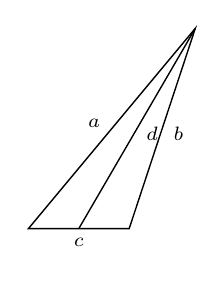
\begin{tikzpicture}[scale=.8]
  \draw[line width=.5pt] (0,0)--(1.6,0)--(2.65,3.18)--cycle;
  \draw[line width=.5pt] (.8,0)--(2.65,3.18);
  \node[font=\scriptsize,above left=-1pt] at (1.25,1.5) {$a$};
  \node[font=\scriptsize,right] at (1.72,1.5) {$d$};
  \node[font=\scriptsize,right] at (2.15,1.5) {$b$};
  \node[font=\scriptsize,below] at (.8,0) {$c$};
\end{tikzpicture}
\end{center}
\end{exercise}

\begin{exercise}
Fix a positive integer $n$. The \emph{Laplacian} $\Delta p$ of a twice
differentiable real-valued function $p$ on $\R^n$ is the function on $\R^n$
defined by
\[ \Delta p = \frac{\partial^2p}{\partial x_1^2}+\cdots
   +\frac{\partial^2p}{\partial x_n^2}. \]
The function $p$ is called \emph{harmonic} if $\Delta p=0$.

A \emph{polynomial} on $\R^n$ is a linear combination (with coefficients in
$\R$) of functions of the form $x_1^{m_1}\cdots x_n^{m_n}$, where
$m_1,\dots,m_n$ are nonnegative integers.

Suppose $q$ is a polynomial on $\R^n$. Prove that there exists a harmonic
polynomial $p$ on $\R^n$ such that $p(x)=q(x)$ for every $x\in\R^n$ with
$\norm{x}=1$.
\exnote{The only fact about harmonic functions that you need for this exercise
is that if $p$ is a harmonic function on $\R^n$ and $p(x)=0$ for all
$x\in\R^n$ with $\norm{x}=1$, then $p=0$.}
\exnote{Hint: A reasonable guess is that the desired harmonic polynomial $p$ is
of the form $q+(1-\norm{x}^2)r$ for some polynomial $r$. Prove that there is a
polynomial $r$ on $\R^n$ such that $q+(1-\norm{x}^2)r$ is harmonic by defining
an operator $T$ on a suitable vector space by
\[ Tr = \Delta\bigl((1-\norm{x}^2)r\bigr) \]
and then showing that $T$ is injective and hence surjective.}
\end{exercise}
\end{exc}

\axquote{In realms of numbers, where the secrets lie,\\
A noble truth emerges from the deep,\\
Cauchy and Schwarz, their wisdom they apply,\\
An inequality for all to keep.\par
Two vectors, by this bond, are intertwined,\\
As inner products weave a gilded thread,\\
Their magnitude, by providence, confined,\\
A bound to which their destiny is wed.\par
Though shadows fall, and twilight dims the day,\\
This inequality will stand the test,\\
To guide us in our quest, to light the way,\\
And in its truth, our understanding rest.\par
So sing, ye muses, of this noble feat,\\
Cauchy--Schwarz, the bound that none can beat.}{written by ChatGPT with input
\emph{Shakespearean sonnet on Cauchy--Schwarz inequality}}
